\documentclass[11pt]{article}

\usepackage{verbatim}
\usepackage{indentfirst}
\usepackage{algorithm2e}
\usepackage{amsmath, amsthm, graphicx, caption}
\usepackage{float}
\usepackage[margin=1in]{geometry}
\newtheorem{theorem}{Theorem}
\numberwithin{theorem}{subsection}
%\newtheorem{algorithm}[theorem]{Algorithm}
\newtheorem{lemma}[theorem]{Lemma}
\newtheorem{definition}[theorem]{Definition}
\newcommand{\optcost}{\text{Optcost}}
\title{Keys Under the Welcome Mat}
\author{Michelle Wang, Matthew Furtney, Andrew Hyer, Michael Xu}

\begin{document}
\maketitle

\section{Snapchat Flaws}

The inspiration for this project was a description of a security flaw in Snapchat, published on the internet.\cite{1}

Snapchat encrypts images that the owner of the device it's running on is not supposed to be able to access.  Unfortunately,
it encrypts them using the hard-coded encryption key ``M02cnQ51Ji97vwT4''.  Once this key is found and known, you can use it
to decrypt these images, accessing images you're not meant to be able to see.

\section{Bulk Analysis}

% Assumes a description of the SnapChat vulnerability
  Inspired by Snapchat's snafu, we strove to find similar errors in other popular apps. We downloaded
$917$ popular Android applications in .apk form for analysis. We summarize our method and results below.

\subsection{Previous Work}

  As one may expect, we were not the first to analyze android apks for security vulnerabilities.
Cryptolint was a system designed by researchers at CMU and UCSB to analyze android apps for security vulnerabilities. 
Cryptolint uses software called Androguard for sophisticated static analysis of the decompiled Android apks.
It checks for six specific types of vulnerabilities: 

\begin{enumerate}
  \item ECB mode of block cipher operation
  \item Constant initialization vectors
  \item Constant encryption keys
  \item Static salts for Password-Based Encryption
  \item Fewer than 1000 iterations of Password-Based Encryption
  \item Constant seeds for SecureRandom()
\end{enumerate}

Unfortunately, we could not locate any source for Cryptolint. Cryptolint's site allows for submission of
applications to be analyzed, but the analyzer did not return any results for us.  The source code of their
system is not available, so we cannot use it for ourselves.   Moreover, the site only supplies $5$ analyzed apps, 
none of them very prominent or popular. 

Given these issues, and given our inability to find any other analysis of such apps, we feel justified in designing 
and coding our own analyzer.

\subsection{Implementation}
We downloaded Android APKs from various locations across the Internet, most notably (\#TODO). Once downloaded, we used
the open-source program APKTool \cite{APKTool} to decompile these APKs.  APKTool decompiles the app into Smali code; this
is the language used by the Android system.
We decompiled all $917$ on a single quad-core machine. In addition to the Smali code, this process generated extraneous files
such as images, sound or fonts. 
  Our next step was to scan the directory and filter the source for relevant strings. We used the \texttt{egrep} to search
each directory for lines in Smali files containing ``const-string''. We fed these lines into a Python script
which checked validity based on Shannon entropy, length, and composition (letters and numbers). Before filtering a
decompiled application averaged $200,000$ lines of Smali code. After filtering, we obtained on average only a few dozen
possible hits for each app.

\subsection{Initial Results}

  We focused on searching for \texttt{const-string} objects, or hardcoded strings, in the decompiled Smali.
At first, we focused on searching for purely high-entropy constant strings of significant length. 
After examining the initial analysis data, we noticed that a large number of cryptographic terms other than keys were being
listed. For example, ``SHA1withRSA'' was a common term that qualified as ``high-entropy''. In light of this discovery,
we decided to investigate references to cryptographic algorithms; while seeing that an app contains the string ``SHA1withRSA''
does not uncover any actual security flaws, it does tell you something about what encryption system the app uses.

\subsection{Aggregate Information}

  Investigating the frequency of cryptographic algorithms yielded some interesting information. We can use
files with a high number of references to pinpoint security hotspots in an application. Additionally, 
cryptographic libraries leave an easily recognizable pattern of crypto references. A quick scan
of our analyzed data reveals that $16$ or $17$ applications make us of the BouncyCastle/SpongyCastle crypto
libraries. The insight here is that we can easily identify which files contains crypto code and check
for hardcoded keys and other vulnerabilities in close proximity.

\subsubsection{Cryptography References}

  Later, we shifted to searching for specific calls to symmetric block cipher methods. We looked for both
block cipher standards and modes such as \textbf{AES}, \textbf{DES}, \textbf{CFB} and \textbf{CBC}. Regex expressions were used to filter
for spurious hits; a string that simply contained \textbf{AES} would not be included. We verified this manually by printing out discovered
references. All the references we inspected were of the format \texttt{AES/CBC/NoPadding} or something similar, which represents
a call to a function from Java's \texttt{Cipher} class in the \texttt{Javax/Crypto} package. Developers who did not use this library for
ciphers may not have been listed, but again our goal was broad trends over a large number of apps. By doing this analysis, we were effectively
examining how a significant proportion of application developers were using block ciphers, and if they were using them correctly.

\begin{figure}[H]
  \caption{References of cryptographic algorithms in $917$ analyzed applications.}
  \centering
  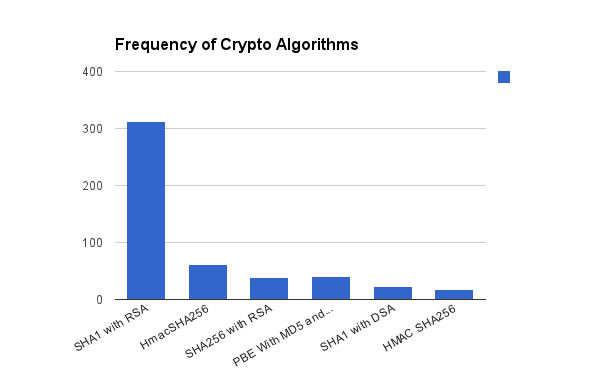
\includegraphics[scale=0.8]{fig1.png}
\end{figure}

\subsubsection{Block Ciphers}

The results we obtained, summarized in Figure 2., are somewhat shocking. We recorded $132$ individual applications which used
\textbf{DES} for their encryption. \textbf{DES} is an antiquated symmetric block cipher standard which relies on $56$ bit keys,
easily brute forceable with modern hardware. While developers may have reasons for using \textbf{DES}, we want to encourage
the community to switch to \textbf{AES} for all symmetric block cipher applications. The benefits of secure cryptography far
outweight convenience or other justifications. We also draw attention to the number of applications that utilize ciphers in
\textbf{ECB} mode. For anything more than a single block, \textbf{ECB} mode is insecure, since each block will always decrypt
in the same way. This essentially leaves the pattern of the plaintext intact, leaking significant information. The canonical
example of this is \textbf{ECB} mode encryption applied to an image of Tux, the Linux penguin. The encrypted data
clearly reveals the outline of Tux. Any area of uniform color is immediately obvious after \textbf{ECB} encryption.
While not entirely comprehensive, our data shows a striking number of applications that use block ciphers in vulnerable
configurations.

\begin{figure}[H]
  \caption{References of Block Cipher Uses in $917$ analyzed applications.}
  \centering
  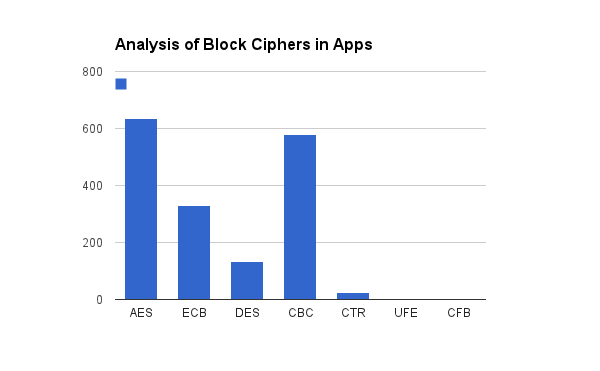
\includegraphics[scale=0.8]{fig2.png}
\end{figure}

\subsection{Back to Snapchat?}

When we ran our basic Python analyzer on Snapchat, we got some interesting results: see Figure 1 (\#TODO).

The key ``M02cnQ51Ji97vwT4'' is, as we would hope, visible here.  However, there are several other sets of
hardcoded strings that look like they could also be keys!  We looked into these, and found some interesting stuff.

There were six keys in the output that looked like they might merit attention:

\begin{itemize}
\item Two strings that look like random keys, in a file called ``RequestAuthorization''. 
\begin{itemize}
\item "iEk21fuwZApXlz93750dmW22pw389dPwOk"
\item "m198sOkJEn37DjqZ32lpRu76xmw288xSQ9"
\end{itemize}
\item Four strings that look like poorly generated passwords, in a file called ``NotificationReciever''.
\begin{itemize}
\item "2peacheszxcsnapchat88whdsb3243"
\item "2ballfacechillahzx8vhf8hh83243"
\item "2baaawnburb1f3dndddhh83243"
\item "2c00l4sk00l88vhfwkipqoewm83243"
\end{itemize}
\end{itemize}

We first Googled these strings to see if they were known of.  The first two keys were: they represent \textbf{another} security
flaw in Snapchat, by which you can access the phone numbers of all Snapchat users and create arbitrary numbers of 'dummy' users.\cite{2}

The four strings that looked like poorly done passwords, however, were not found anywhere on the Internet.  We investigated the file
they came from to see if there was anything interesting in there: see Figure 2(\#TODO)

The code here is in Smali, which is difficult to read, but what's going on on this page is simple enough.  Four integer fields (designated by
letters ``a'' through ``d'' in the decompiled code) are initialized at the top.  Each of the four strings we found is hashed into an int, which 
is inserted into one of those fields.

This means that those integer fields are functionally hard-coded themselves; while their values are recalculated every time, they're recalculated in a
deterministic way from hardcoded inputs, and so will always be the same.

\subsection{Continued Investigation}

\subsection{Potential Applications}

We think there are a lot of potential future applications to the idea of making users aware of the security (or lack thereof) of apps they use.  We
cannot think of a better example of this than that presented by Snapchat; Snapchat currently has millions of users, who are using it under the
mistaken impression that it provides security.  Given that there are two separate critical security flaws in Snapchat avaiable online (and given that
each of them has been online for months or more, with no response from Snapchat), and given our own findings, we think that Snapchat's users are being
rather badly misled by Snapchat's claims of 'security'.

\subsection{Responsible Disclosure}

When considering vulnerabilities in published software, it is important to be careful not to release anything that will harm software manufacturers.
Through most of our paper, however, we deal with these flaws only in aggregate; we are not mentioning specific apps, only classes of security
flaw that we have observed throughout many apps.  This isn't a significant security issue; these flaws are already known, all we have done is
data gathering to determine how frequent they are.

We have gone into some detail on the security flaws of Snapchat.  However, as many such flaws are already public knowledge\cite{1}\cite{2}, we do
not think it is necessary to contrain the publication of this piece on that basis.

\begin{thebibliography}{9}

        \bibitem{1}
        http://security.stackexchange.com/questions/52584/why-can-we-still-crack-snapchat-photos-in-12-lines-of-ruby
        \bibitem{2}
        http://gibsonsec.org/snapchat/snapchat\_gibsonsec.txt
        \bibitem{APKTool}
        https://code.google.com/p/android-apktool/

\end{thebibliography}
\end{document}
